\documentclass[aspectratio=169]{beamer}

% Theme and Color Setup
\usetheme{Madrid}
\usecolortheme{whale}
\useinnertheme{rectangles}
\useoutertheme{miniframes}

% Additional Packages
\usepackage[utf8]{inputenc}
\usepackage[T1]{fontenc}
\usepackage{graphicx}
\usepackage{booktabs}
\usepackage{listings}
\usepackage{amsmath}
\usepackage{amssymb}
\usepackage{xcolor}
\usepackage{tikz}
\usepackage{pgfplots}
\pgfplotsset{compat=1.18}
\usetikzlibrary{positioning}
\usepackage{hyperref}

% Custom Colors
\definecolor{myblue}{RGB}{31, 73, 125}
\definecolor{mygray}{RGB}{100, 100, 100}
\definecolor{mygreen}{RGB}{0, 128, 0}
\definecolor{myorange}{RGB}{230, 126, 34}
\definecolor{mycodebackground}{RGB}{245, 245, 245}

% Set Theme Colors
\setbeamercolor{structure}{fg=myblue}
\setbeamercolor{frametitle}{fg=white, bg=myblue}
\setbeamercolor{title}{fg=myblue}
\setbeamercolor{section in toc}{fg=myblue}
\setbeamercolor{item projected}{fg=white, bg=myblue}
\setbeamercolor{block title}{bg=myblue!20, fg=myblue}
\setbeamercolor{block body}{bg=myblue!10}
\setbeamercolor{alerted text}{fg=myorange}

% Set Fonts
\setbeamerfont{title}{size=\Large, series=\bfseries}
\setbeamerfont{frametitle}{size=\large, series=\bfseries}
\setbeamerfont{caption}{size=\small}
\setbeamerfont{footnote}{size=\tiny}

% Custom Commands
\newcommand{\hilight}[1]{\colorbox{myorange!30}{#1}}
\newcommand{\concept}[1]{\textcolor{myblue}{\textbf{#1}}}
\newcommand{\separator}{\begin{center}\rule{0.5\linewidth}{0.5pt}\end{center}}

% Title Page Information
\title[Introduction to RL]{Week 12: Introduction to Reinforcement Learning}
\author[J. Smith]{John Smith, Ph.D.}
\institute[University Name]{
  Department of Computer Science\\
  University Name\\
  \vspace{0.3cm}
  Email: email@university.edu\\
  Website: www.university.edu
}
\date{\today}

% Document Start
\begin{document}

\frame{\titlepage}

\begin{frame}[fragile]
    \frametitle{Introduction to Reinforcement Learning}
    \begin{block}{What is Reinforcement Learning (RL)?}
        Reinforcement Learning (RL) is a branch of machine learning where an agent learns to make decisions by performing tasks in an environment. The agent receives feedback in the form of rewards or penalties based on its actions.
    \end{block}
    
    \begin{block}{Key Concepts}
        \begin{itemize}
            \item \textbf{Agent}: The learner or decision maker (e.g., a robot or software algorithm).
            \item \textbf{Environment}: The context in which the agent operates (e.g., a game or real-world scenarios).
            \item \textbf{Action (A)}: All possible moves the agent can make in the environment.
            \item \textbf{State (S)}: The current configuration of the environment.
            \item \textbf{Reward (R)}: A numerical value received after performing an action, reflecting its effectiveness.
        \end{itemize}
    \end{block}
\end{frame}

\begin{frame}[fragile]
    \frametitle{The Learning Process}
    The RL process involves the following cycle:
    \begin{enumerate}
        \item \textbf{Observation}: The agent observes the current state (S) of the environment.
        \item \textbf{Action}: The agent selects an action (A) based on the observed state.
        \item \textbf{Reward}: After performing the action, the agent receives a reward (R) and transitions to a new state (S').
        \item \textbf{Update}: The agent updates its knowledge or policy based on the reward to improve future actions.
    \end{enumerate}
\end{frame}

\begin{frame}[fragile]
    \frametitle{Significance in AI}
    \begin{block}{Importance of RL}
        \begin{itemize}
            \item \textbf{Autonomous Learning}: RL allows agents to learn optimal strategies without explicit programming.
            \item \textbf{Applications}:
                \begin{itemize}
                    \item \textbf{Gaming}: AI systems mastering games by learning strategies (e.g., AlphaGo).
                    \item \textbf{Robotics}: Learning navigation and task performance in dynamic environments.
                    \item \textbf{Finance}: Optimizing portfolio management through algorithmic trading.
                    \item \textbf{Healthcare}: Personalizing treatment paths based on patient feedback.
                \end{itemize}
        \end{itemize}
    \end{block}
    
    \begin{block}{Example: Game Playing}
        Consider an agent in a maze:
        The agent receives positive rewards for reaching the goal and negative rewards for hitting walls, learning optimal paths over time.
    \end{block}
\end{frame}

\begin{frame}[fragile]{What is Reinforcement Learning? - Part 1}
    \frametitle{Definition of Reinforcement Learning (RL)}
    \begin{block}{Definition}
        Reinforcement Learning (RL) is a machine learning paradigm where an agent learns to make decisions by taking actions in an environment to maximize cumulative rewards.
    \end{block}
    \begin{block}{Key Differences from Supervised Learning}
        Unlike traditional supervised learning, where the model learns from labeled data (input-output pairs), RL focuses on learning from the consequences of actions.
    \end{block}
\end{frame}

\begin{frame}[fragile]{What is Reinforcement Learning? - Part 2}
    \frametitle{Distinct Characteristics of Reinforcement Learning}
    \begin{itemize}
        \item \textbf{Agent and Environment}
            \begin{itemize}
                \item \textbf{Agent}: The learner or decision-maker.
                \item \textbf{Environment}: The setting where the agent operates.
            \end{itemize}
            \textit{Example: In chess, the player (agent) makes moves (actions) on the chessboard (environment).}
            
        \item \textbf{Exploration vs. Exploitation}
            \begin{itemize}
                \item \textbf{Exploration}: Trying new actions for potential rewards.
                \item \textbf{Exploitation}: Using known actions that have yielded high rewards.
            \end{itemize}
            \textit{Key Point: Balancing exploration and exploitation is crucial.}
            
        \item \textbf{Delayed Rewards}
            \begin{itemize}
                \item Rewards may be received after a series of actions, complicating learning.
            \end{itemize}
            \textit{Example: In video games, points are awarded for completing goals that result from earlier actions.}
    \end{itemize}
\end{frame}

\begin{frame}[fragile]{What is Reinforcement Learning? - Part 3}
    \frametitle{Comparison with Other Learning Paradigms}
    \begin{itemize}
        \item \textbf{Feedback Loop}
            \begin{itemize}
                \item The agent updates its knowledge dynamically based on rewards.
            \end{itemize}
        
        \item \textbf{State Representation}
            \begin{itemize}
                \item The agent observes the current state, influencing its decisions.
            \end{itemize}
            \textit{Example: A robot's sensors indicate its position and direction.}
            
        \item \textbf{Summary of Learning Types}
            \begin{itemize}
                \item \textbf{Supervised Learning}: Learns from labeled data (e.g., predicting house prices).
                \item \textbf{Unsupervised Learning}: Learns from unlabeled data (e.g., clustering customers).
            \end{itemize}
        
        \item \textbf{Final Thought}
            \begin{itemize}
                \item RL focuses on long-term rewards, setting it apart from other learning methods.
            \end{itemize}
    \end{itemize}
\end{frame}

\begin{frame}[fragile]
    \frametitle{Components of Reinforcement Learning}
    \begin{block}{Learning Objectives}
        By the end of this slide, you should be able to:
        \begin{enumerate}
            \item Describe the fundamental components of Reinforcement Learning (RL).
            \item Differentiate between the roles of the agent, environment, actions, and states.
            \item Illustrate how these components interact within a typical RL setup.
        \end{enumerate}
    \end{block}
\end{frame}

\begin{frame}[fragile]
    \frametitle{Key Components of Reinforcement Learning}
    \begin{itemize}
        \item \textbf{Agent:} 
            \begin{itemize}
                \item Definition: The learner or decision-maker in an RL setting. The goal is to maximize cumulative reward.
                \item Example: In a game of chess, the player is the agent making moves to win.
            \end{itemize}
        \item \textbf{Environment:} 
            \begin{itemize}
                \item Definition: Everything the agent interacts with, providing feedback in the form of rewards or penalties.
                \item Example: The chessboard and the rules of chess are the environment.
            \end{itemize}
    \end{itemize}
\end{frame}

\begin{frame}[fragile]
    \frametitle{Key Components of Reinforcement Learning (contd.)}
    \begin{itemize}
        \item \textbf{Actions:} 
            \begin{itemize}
                \item Definition: The set of all possible moves the agent can make in the environment at any state.
                \item Example: Actions in chess include moving a pawn forward or capturing a piece.
                \item Formula: The action space can be represented as a set \( A = \{a_1, a_2, \ldots, a_n\} \).
            \end{itemize}
        \item \textbf{States:} 
            \begin{itemize}
                \item Definition: The current situation of the environment as perceived by the agent, containing all necessary information.
                \item Example: A state in chess is defined by the arrangement of pieces on the board.
                \item Representation: States denoted as \( S_t \) for the state at time \( t \).
            \end{itemize}
    \end{itemize}
\end{frame}

\begin{frame}[fragile]
    \frametitle{Interactions Among Components}
    \begin{itemize}
        \item \textbf{Transition:} The process where the agent takes action \( a \) in state \( S \) leading to new state \( S' \), often modeled with:
        \[
        P(S' | S, a)
        \]
        \item \textbf{Feedback Loop:} The environment gives the agent a reward \( R \) based on the action, which helps the agent improve its future decisions.
    \end{itemize}
\end{frame}

\begin{frame}[fragile]
    \frametitle{Summary and Next Topic}
    \begin{block}{Summary}
        Reinforcement Learning consists of four main components - the agent, environment, actions, and states - that interact dynamically to facilitate learning. Understanding these elements is crucial for grasping how RL algorithms operate to solve complex problems.
    \end{block}
    
    \begin{block}{Next Topic Preview}
        In the next slide, we will explore the concept of rewards in RL and their significance in guiding the agent's learning process.
    \end{block}
\end{frame}

\begin{frame}[fragile]
    \frametitle{Rewards in Reinforcement Learning - Understanding Rewards}
    In Reinforcement Learning (RL), \textbf{rewards} serve as the primary feedback signal that an agent receives from the environment after taking an action. 
    \begin{itemize}
        \item Rewards indicate how good or bad an action is in achieving a specific goal.
        \item This feedback drives the agent's learning process, guiding it to improve its performance over time.
    \end{itemize}
\end{frame}

\begin{frame}[fragile]
    \frametitle{Rewards in Reinforcement Learning - Types of Rewards}
    There are several types of rewards that influence an agent's learning:
    \begin{enumerate}
        \item \textbf{Immediate Rewards}
        \begin{itemize}
            \item Received right after performing an action.
            \item Example: In a game, scoring points for a correct move.
        \end{itemize}
        
        \item \textbf{Cumulative Rewards (Return)}
        \begin{itemize}
            \item Total expected reward over time, including future rewards discounted by their delay.
            \item Formula: 
            \begin{equation}
            G_t = r_t + \gamma r_{t+1} + \gamma^2 r_{t+2} + \ldots
            \end{equation}
        \end{itemize}
        
        \item \textbf{Delayed Rewards}
        \begin{itemize}
            \item Rewards not received immediately after an action, requiring the agent to track past actions.
            \item Example: In chess, points may be awarded only after winning the game.
        \end{itemize}
        
        \item \textbf{Sparse Rewards}
        \begin{itemize}
            \item Rewards that occur infrequently, making learning challenging.
            \item Example: Finding a treasure, with the reward given only upon completion.
        \end{itemize}
    \end{enumerate}
\end{frame}

\begin{frame}[fragile]
    \frametitle{Rewards in Reinforcement Learning - Impact on Learning}
    The structure of rewards has a significant impact on agent learning:
    \begin{itemize}
        \item \textbf{Learning Dynamics}: A well-defined reward structure can lead to quicker mastery of tasks.
        \item \textbf{Exploration vs. Exploitation}: Balancing known rewarding actions with the exploration of new actions is crucial. Poorly designed rewards might cause the agent to over-exploit suboptimal strategies.
        \item \textbf{Rewards Shaping}: Modifying the structure or frequency of rewards can improve learning and convergence rates.
    \end{itemize}
    
    \textbf{Key Points to Emphasize:}
    \begin{itemize}
        \item Rewards are the cornerstone of an agent's learning process.
        \item Differentiating types of rewards aids in shaping effective learning strategies.
        \item The agent's performance heavily depends on reward structures.
    \end{itemize}
\end{frame}

\begin{frame}[fragile]
    \frametitle{Conclusion}
    Understanding how rewards function in RL is crucial for designing intelligent systems. 
    By carefully crafting rewards, we can significantly enhance an agent's learning capabilities and overall performance in its tasks.
\end{frame}

\begin{frame}[fragile]
    \frametitle{Policies in Reinforcement Learning}
    \begin{block}{What is a Policy?}
        In Reinforcement Learning (RL), a \textbf{policy} is a strategy used by an agent to determine its actions based on the current state of the environment. 
    \end{block}
    \begin{itemize}
        \item Defines the relationship between states and actions.
        \item For every state, the policy outlines what action the agent should take.
    \end{itemize}
\end{frame}

\begin{frame}[fragile]
    \frametitle{Policies in Reinforcement Learning - Mathematical Definition}
    \begin{itemize}
        \item \textbf{Deterministic Policy}: \( \pi: S \rightarrow A \)
        \item \textbf{Stochastic Policy}: \( \pi(a|s) = P(A = a | S = s) \)
    \end{itemize}
    Where:
    \begin{itemize}
        \item \( S \) is the set of all possible states.
        \item \( A \) is the set of all possible actions.
    \end{itemize}
\end{frame}

\begin{frame}[fragile]
    \frametitle{Types of Policies}
    \begin{enumerate}
        \item \textbf{Deterministic Policy}
            \begin{itemize}
                \item Selects the same action for a given state every time.
                \item \textbf{Example}: If the state is "Hungry", the agent always chooses "Eat".
            \end{itemize}
        \item \textbf{Stochastic Policy}
            \begin{itemize}
                \item Selects actions based on a probability distribution over actions.
                \item \textbf{Example}: In the state "Hungry", the agent might choose "Eat" with a probability of 0.8 and "Drink" with a probability of 0.2.
            \end{itemize}
    \end{enumerate}
\end{frame}

\begin{frame}[fragile]
    \frametitle{How Policies Govern Agent Behavior}
    \begin{itemize}
        \item A policy directs an agent's decision-making process.
        \item Influences the effectiveness in achieving goals based on feedback.
        \item Evaluated based on the \textbf{cumulative rewards} and \textbf{Expected Return}.
    \end{itemize}
    \begin{equation}
        R_t = r_t + \gamma r_{t+1} + \gamma^2 r_{t+2} + \ldots
    \end{equation}
    Where:
    \begin{itemize}
        \item \( R_t \) is the total return starting from time \( t \).
        \item \( r_t \) is the immediate reward after taking action \( a_t \).
        \item \( \gamma \) is the discount factor.
    \end{itemize}
\end{frame}

\begin{frame}[fragile]
    \frametitle{Example Scenario}
    \begin{itemize}
        \item \textbf{Environment}: A maze where an agent needs to find the exit.
        \item \textbf{States}: Different positions within the maze.
        \item \textbf{Actions}: Move Up, Down, Left, Right.
        \item \textbf{Policy}: Maps each position to specific actions with associated probabilities.
    \end{itemize}
    \begin{block}{Visualization of Policies}
        \begin{itemize}
            \item A grid representing the maze. 
            \item Each cell is a state, and arrows depict preferred action(s).
            \item Arrow length indicates action selection probability.
        \end{itemize}
    \end{block}
\end{frame}

\begin{frame}[fragile]
    \frametitle{Key Points and Conclusion}
    \begin{itemize}
        \item Policies are foundational to agents' learning in RL.
        \item Policy optimization is critical, with methods like Policy Gradients and Q-Learning.
    \end{itemize}
    \begin{block}{Conclusion}
        Understanding policies prepares us for the next topic: \textbf{Exploration vs. Exploitation}!
    \end{block}
\end{frame}

\begin{frame}[fragile]
    \frametitle{Exploration vs. Exploitation}
    \begin{block}{Learning Objectives}
        \begin{itemize}
            \item Understand the concepts of exploration and exploitation in Reinforcement Learning.
            \item Recognize the importance of balancing between trying new actions (exploration) and leveraging existing knowledge (exploitation).
            \item Identify challenges and strategies to manage the exploration-exploitation trade-off.
        \end{itemize}
    \end{block}
\end{frame}

\begin{frame}[fragile]
    \frametitle{Key Concepts}
    \begin{block}{Exploration}
        \begin{itemize}
            \item Refers to the agent's behavior of trying new actions that may yield different rewards.
            \item Purpose: Discovering potentially better strategies that have not been tried yet.
            \item Example: In a maze, exploring new paths that haven't been taken might lead to finding the exit faster.
        \end{itemize}
    \end{block}
    
    \begin{block}{Exploitation}
        \begin{itemize}
            \item Involves leveraging the current knowledge to maximize rewards from known actions.
            \item Purpose: Utilizes learned behaviors and strategies that are already proven to work effectively.
            \item Example: If a specific path in the maze consistently leads to food, the agent will use that path instead of trying new ones.
        \end{itemize}
    \end{block}
\end{frame}

\begin{frame}[fragile]
    \frametitle{The Exploration-Exploitation Dilemma}
    \begin{itemize}
        \item Striking a balance between exploration and exploitation is crucial for optimizing long-term rewards.
        \item Too much exploration can lead to insufficient learning (spending too much time on potentially less effective actions).
        \item Too much exploitation can miss out on better opportunities and lead to a suboptimal policy.
    \end{itemize}
\end{frame}

\begin{frame}[fragile]
    \frametitle{Strategies to Manage the Trade-Off}
    \begin{enumerate}
        \item \textbf{Epsilon-Greedy Strategy:}
            \begin{itemize}
                \item With probability $\epsilon$, choose a random action (exploration), and with probability $(1-\epsilon)$, choose the best-known action (exploitation).
                \item Example: If $\epsilon = 0.1$, there’s a 10\% chance of trying a new action and a 90\% chance of selecting the best-known one.
            \end{itemize}
        
        \item \textbf{Softmax Selection:}
            \begin{itemize}
                \item Actions are selected according to a probability distribution derived from their estimated values, favoring higher-value actions.
                \item Encourages exploration while still leaning towards rewarding actions based on their probabilities.
            \end{itemize}
        
        \item \textbf{Upper Confidence Bound (UCB):}
            \begin{itemize}
                \item Selects actions based not only on their average rewards but also on the uncertainty associated with them, promoting exploration of less tried actions.
            \end{itemize}
    \end{enumerate}
\end{frame}

\begin{frame}[fragile]
    \frametitle{Visual Representation}
    \begin{center}
        \textbf{Exploration vs. Exploitation Space}
        
        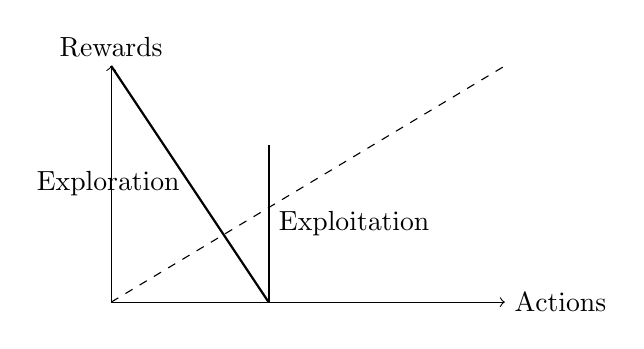
\begin{tikzpicture}
            \draw[->] (0,0) -- (0,3) node[above] {Rewards};
            \draw[->] (0,0) -- (5,0) node[right] {Actions};
            \draw[thick] (2,0) -- (2,2) node[midway, right] {Exploitation};
            \draw[thick] (2,0) -- (0,3) node[midway, left] {Exploration};
            \draw[dashed] (0,0) -- (5,3);
        \end{tikzpicture}
    \end{center}
\end{frame}

\begin{frame}[fragile]
    \frametitle{Conclusion}
    \begin{itemize}
        \item The balance between exploration and exploitation is vital in Reinforcement Learning.
        \item Through strategies like epsilon-greedy and UCB, agents can learn a more effective policy leading to better decision-making over time.
        \item Understanding when to explore or exploit helps maximize overall rewards and improve learning efficiency.
    \end{itemize}
    
    *Next Slide: Q-Learning Basics - Overview of Q-Learning as a foundational RL algorithm and introduction to the Q-table.*
\end{frame}

\begin{frame}[fragile]
    \frametitle{Q-Learning Basics}
    \begin{block}{Learning Objectives}
        \begin{enumerate}
            \item Understand the fundamentals of Q-Learning as a key algorithm in Reinforcement Learning (RL).
            \item Learn how the Q-table is structured and used to inform decision-making.
        \end{enumerate}
    \end{block}
\end{frame}

\begin{frame}[fragile]
    \frametitle{What is Q-Learning?}
    \begin{itemize}
        \item Q-Learning is a model-free reinforcement learning algorithm that learns the value of an action in a given state.
        \item The goal is to maximize cumulative rewards for the agent through its actions in an environment.
        \begin{itemize}
            \item \textbf{Model-Free:} No model of the environment is required; learning is based on direct experiences.
            \item \textbf{Off-Policy:} It learns about the optimal policy while exploring with a different policy.
        \end{itemize}
    \end{itemize}
\end{frame}

\begin{frame}[fragile]
    \frametitle{Key Concepts and Q-Values}
    \begin{block}{Key Concepts}
        \begin{itemize}
            \item \textbf{Agent:} The decision-maker that seeks to maximize rewards.
            \item \textbf{Environment:} The context in which the agent operates, defined by states and actions.
            \item \textbf{States (S):} All possible situations in which an agent can find itself.
            \item \textbf{Actions (A):} All possible moves the agent can make within a state.
        \end{itemize}
    \end{block}
    
    \begin{block}{Q-Values}
        The \textbf{Q-value} for a state-action pair, denoted as \( Q(s, a) \), represents the expected future rewards that an agent can obtain by taking action \( a \) in state \( s \) and then following the optimal policy thereafter.
    \end{block}
\end{frame}

\begin{frame}[fragile]
    \frametitle{The Q-Table}
    The Q-table is a key component of Q-Learning, where each entry corresponds to a state-action pair.
    
    \begin{block}{Structure}
        \begin{itemize}
            \item \textbf{Rows:} Represent states (s)
            \item \textbf{Columns:} Represent actions (a)
            \item \textbf{Each cell:} Contains the Q-value for the respective state-action pair
        \end{itemize}
    \end{block}

    \begin{block}{Example Q-Table} 
        \begin{tabular}{|c|c|c|c|}
            \hline
            State (S) & Action 1 (A1) & Action 2 (A2) & Action 3 (A3) \\
            \hline
            S1 & 0.5 & 0.2 & 0.3 \\
            S2 & 0.4 & 0.8 & 0.1 \\
            S3 & 0.6 & 0.3 & 0.9 \\
            \hline
        \end{tabular}
    \end{block}
\end{frame}

\begin{frame}[fragile]
    \frametitle{Q-Learning Algorithm}
    \begin{enumerate}
        \item \textbf{Initialize} the Q-table with arbitrary values.
        \item For each episode:
            \begin{itemize}
                \item \textbf{Choose} an action using a policy (e.g., $\epsilon$-greedy).
                \item \textbf{Perform} the action and observe the reward and next state.
                \item \textbf{Update the Q-value} using the formula:
                \[
                Q(s, a) \leftarrow Q(s, a) + \alpha \left( r + \gamma \max_{a'} Q(s', a') - Q(s, a) \right)
                \]
            \end{itemize}
        \item Where:
        \begin{itemize}
            \item \( \alpha \) = Learning rate (0 < \( \alpha \) ≤ 1)
            \item \( r \) = Reward received
            \item \( \gamma \) = Discount factor (0 ≤ \( \gamma \) < 1)
            \item \( s' \) = New state after action
            \item \( a' \) = Possible actions in state \( s' \)
        \end{itemize}
    \end{enumerate}
\end{frame}

\begin{frame}[fragile]
    \frametitle{Key Points and Conclusion}
    \begin{itemize}
        \item Q-Learning's independence from the environment model allows for adaptability to changes.
        \item The balance between exploration and exploitation is crucial for effective learning.
        \item The Q-table can become excessively large with many states and actions, necessitating advanced techniques like function approximation (e.g., deep Q-networks).
    \end{itemize}

    \begin{block}{Conclusion}
        Q-Learning is a foundational algorithm in reinforcement learning that supports optimal decision-making through the use of a Q-table. This understanding serves as a foundation for exploring more complex RL topics, like Markov Decision Processes (MDPs), which will be discussed in the next slide.
    \end{block}
\end{frame}

\begin{frame}[fragile]
    \frametitle{Markov Decision Processes (MDPs) - Introduction}
    \begin{block}{Introduction}
        A \textbf{Markov Decision Process (MDP)} is a mathematical framework for modeling decision-making in Reinforcement Learning (RL). It describes how agents make decisions to maximize cumulative rewards.
    \end{block}
\end{frame}

\begin{frame}[fragile]
    \frametitle{Markov Decision Processes (MDPs) - Components}
    \begin{block}{Key Components of MDPs}
        \begin{itemize}
            \item \textbf{States (S)}: Set of possible states.
            \item \textbf{Actions (A)}: Set of actions available to the agent.
            \item \textbf{Transition Probability (P)}: Probability of moving from one state to another. 
                \begin{equation}
                P(s' | s, a)
                \end{equation}
            \item \textbf{Rewards (R)}: Feedback from actions.
            \item \textbf{Discount Factor ($\gamma$)}: Importance of future rewards (0 to 1).
        \end{itemize}
    \end{block}
\end{frame}

\begin{frame}[fragile]
    \frametitle{Markov Decision Processes (MDPs) - Decision Making}
    \begin{block}{Decision Making and Bellman Equation}
        The agent follows a \textbf{policy} to decide actions, aiming to learn an optimal policy \( \pi \) for maximum expected return:
        
        \begin{equation}
        V(s) = R(s) + \gamma \sum_{s'} P(s' | s, a)V(s')
        \end{equation}
        
        Where:
        \begin{itemize}
            \item $V(s)$: Value of state $s$.
            \item $R(s)$: Immediate reward after transition from $s$.
        \end{itemize}
    \end{block}
\end{frame}

\begin{frame}[fragile]{Temporal Difference Learning - Overview}
    \begin{block}{Overview}
        Temporal Difference (TD) Learning is a cornerstone of Reinforcement Learning (RL) that combines dynamic programming and Monte Carlo methods. It enables agents to:
        \begin{itemize}
            \item Predict future rewards based on experiences.
            \item Learn without needing a model of the environment.
        \end{itemize}
    \end{block}
\end{frame}

\begin{frame}[fragile]{Temporal Difference Learning - Key Concepts}
    \begin{enumerate}
        \item \textbf{Definition:} 
            TD Learning estimates a state's value using future state values, combining estimation and bootstrapping.
            
        \item \textbf{Temporal Difference Error:} 
            The calculated difference between predicted value and actual reward:
            \begin{equation}
                \delta_t = r_t + \gamma V(s_{t+1}) - V(s_t)
            \end{equation}
            where:
            \begin{itemize}
                \item \( \delta_t \): TD error at time \( t \)
                \item \( r_t \): Reward after action in state \( s_t \)
                \item \( \gamma \): Discount factor (0 ≤ \( \gamma \) < 1)
                \item \( V(s_t) \): Estimated value of current state
                \item \( V(s_{t+1}) \): Estimated value of next state
            \end{itemize}
        
        \item \textbf{Update Rule:} 
            The state value is updated based on the TD error:
            \begin{equation}
                V(s_t) \leftarrow V(s_t) + \alpha \delta_t
            \end{equation}
            where \( \alpha \) is the learning rate.
    \end{enumerate}
\end{frame}

\begin{frame}[fragile]{Temporal Difference Learning - Examples & Applications}
    \begin{block}{Examples}
        \begin{itemize}
            \item \textbf{Game Example:} In Tic-Tac-Toe, agents update state values based on the outcome of moves.
            \item \textbf{Real-World Example:} In finance, TD Learning predicts stock prices using progressively received information.
        \end{itemize}
    \end{block}

    \begin{block}{Applications}
        TD Learning is suitable for:
        \begin{itemize}
            \item Game playing (e.g., AlphaGo)
            \item Robotics for navigation and manipulation
        \end{itemize}
    \end{block}
\end{frame}

\begin{frame}[fragile]{Temporal Difference Learning - Conclusion}
    \begin{block}{Conclusion}
        Temporal Difference Learning is fundamental in RL, enabling agents to:
        \begin{itemize}
            \item Form effective value estimates.
            \item Engage and learn from their environment, leading to improved decision-making.
        \end{itemize}
    \end{block}
\end{frame}

\begin{frame}[fragile]
    \frametitle{Deep Reinforcement Learning}
    \begin{block}{Overview}
        Deep Reinforcement Learning (Deep RL) combines reinforcement learning (RL) principles with deep learning techniques. This powerful paradigm enables agents to learn from high-dimensional sensory inputs in complex environments, such as playing Atari games, driving cars, or managing resources in games like Dota 2.
    \end{block}
\end{frame}

\begin{frame}[fragile]
    \frametitle{Key Concepts in Deep RL}
    \begin{enumerate}
        \item \textbf{Agent}: The learner or decision-maker that interacts with the environment.
        \item \textbf{Environment}: The physical or virtual space within which the agent operates and provides feedback based on actions.
        \item \textbf{State (s)}: Representation of the current situation of the environment.
        \item \textbf{Action (a)}: Decision made by the agent that can affect the environment.
        \item \textbf{Reward (r)}: Scalar feedback signal received after taking an action, indicating success toward a goal.
        \item \textbf{Policy ($\pi$)}: Strategy that defines actions based on the current state.
        \item \textbf{Value Function (V)}: Estimates how good it is to be in a given state, predicting future rewards.
    \end{enumerate}
\end{frame}

\begin{frame}[fragile]
    \frametitle{Neural Networks in Deep RL}
    \begin{block}{Role of Neural Networks}
        Deep learning models, specifically neural networks, play a crucial role in approximating policies and value functions.
    \end{block}
    \begin{itemize}
        \item \textbf{Function Approximation}: Mapping states to actions or state values through many hidden layers.
        \item \textbf{End-To-End Learning}: Learning directly from raw input data (like pixels) to output decisions with minimal preprocessing.
    \end{itemize}
\end{frame}

\begin{frame}[fragile]
    \frametitle{Example: Deep Q-Network (DQN)}
    \begin{block}{Q-Learning Formula}
        In traditional Q-learning, the update rule is:
        \begin{equation}
        Q(s, a) \leftarrow Q(s, a) + \alpha \left[ r + \gamma \max_{a'} Q(s', a') - Q(s, a) \right]
        \end{equation}
        Where:
        \begin{itemize}
            \item $\alpha$: learning rate.
            \item $\gamma$: discount factor.
            \item $s'$: resulting state after taking action $a$.
        \end{itemize}
    \end{block}
    \begin{block}{DQN}
        DQN modifies this by replacing the Q-table with a neural network that predicts Q-values for all actions given a state.
    \end{block}
\end{frame}

\begin{frame}[fragile]
    \frametitle{Key Points to Emphasize}
    \begin{itemize}
        \item \textbf{Generalization}: More generalization to unseen states using neural networks.
        \item \textbf{Experience Replay}: Improves learning efficiency by reusing past experiences stored in a buffer.
        \item \textbf{Stability}: Techniques like target networks stabilize Q-value updates and are pivotal in training Deep RL algorithms.
    \end{itemize}
\end{frame}

\begin{frame}[fragile]
    \frametitle{Challenges and Future Directions}
    \begin{enumerate}
        \item \textbf{Sample Efficiency}: Requires a large amount of data to learn effectively.
        \item \textbf{Exploration vs. Exploitation}: Balancing exploration of new actions and exploiting known rewarding actions is crucial.
        \item \textbf{Safety and Understanding}: Ensuring that Deep RL models operate safely in real-world applications is a significant concern.
    \end{enumerate}
\end{frame}

\begin{frame}[fragile]
    \frametitle{Applications of Reinforcement Learning - Overview}
    \begin{block}{Overview}
        Reinforcement Learning (RL) is a powerful machine learning approach enabling agents to learn optimal behaviors through interactions with their environments.
        This slide explores key real-world applications of RL, highlighting its versatility and relevance across various domains.
    \end{block}
\end{frame}

\begin{frame}[fragile]
    \frametitle{Applications of Reinforcement Learning - Key Applications}
    \begin{itemize}
        \item \textbf{Robotics}
        \begin{itemize}
            \item \textit{Concept}: RL is used in developing intelligent robotic systems that adapt to complex tasks.
            \item \textit{Example}: Boston Dynamics enhances the capabilities of its Spot robot using RL, allowing navigation in dynamic environments.
        \end{itemize}
        
        \item \textbf{Game Playing}
        \begin{itemize}
            \item \textit{Concept}: RL excels in mastering games, often surpassing human performance.
            \item \textit{Example}: AlphaGo from DeepMind learned Go strategies through self-play, achieving victory against a world champion.
        \end{itemize}
        
        \item \textbf{Recommendation Systems}
        \begin{itemize}
            \item \textit{Concept}: RL optimizes user experiences with personalized content recommendations.
            \item \textit{Example}: E-commerce (like Amazon) and streaming services (like Netflix) use RL to recommend products or movies based on user behavior.
        \end{itemize}
    \end{itemize}
\end{frame}

\begin{frame}[fragile]
    \frametitle{Applications of Reinforcement Learning - Key Points}
    \begin{itemize}
        \item \textbf{Adaptability}: RL systems can adapt and optimize actions based on environmental feedback, ideal for dynamic scenarios.
        \item \textbf{Exploration vs. Exploitation}: Agents must balance exploring new strategies to improve and exploiting known strategies to maximize rewards.
        \item \textbf{Real-world Impact}: RL's applications in robotics, gaming, and recommendations demonstrate its potential to revolutionize industries through autonomous, intelligent decision-making.
    \end{itemize}
\end{frame}

\begin{frame}[fragile]
    \frametitle{Applications of Reinforcement Learning - Conclusion}
    Reinforcement Learning applications are diverse and continually expanding, illustrating its capability to tackle complex tasks via interactive learning. A thorough understanding of these applications is essential for appreciating RL's broader implications in shaping future technology.
\end{frame}

\begin{frame}[fragile]
    \frametitle{Challenges in Reinforcement Learning}
    \begin{block}{Overview of Reinforcement Learning (RL)}
        Reinforcement Learning is a type of machine learning where an agent learns to make decisions by taking actions in an environment to maximize cumulative rewards. Unlike supervised learning, there is no explicit dataset; instead, the agent explores and receives feedback from the environment in the form of rewards or penalties based on its actions.
    \end{block}
\end{frame}

\begin{frame}[fragile]
    \frametitle{Challenges in Reinforcement Learning - Part 1}
    \section*{1. Sample Inefficiency}
    \begin{itemize}
        \item \textbf{Definition:} Sample inefficiency refers to the amount of training data or interactions required to learn an effective policy.
        \item \textbf{Explanation:} In RL, learning often requires a vast number of interactions with the environment to collect enough data to improve the agent's policy. This is problematic in environments where collecting samples is expensive or limited.
        \item \textbf{Example:} In a robotic control task, an agent may take hours to learn to reach a target but could achieve only a few successful outcomes due to inefficient exploration.
    \end{itemize}

    \begin{block}{Key Points}
        \begin{itemize}
            \item RL algorithms, like Q-learning, often need hundreds or thousands of episodes to converge to an optimal policy.
            \item The exploration versus exploitation dilemma exacerbates inefficiency, requiring a balance to discover new strategies and refine existing ones.
        \end{itemize}
    \end{block}
\end{frame}

\begin{frame}[fragile]
    \frametitle{Challenges in Reinforcement Learning - Part 2}
    \section*{2. Long Training Times}
    \begin{itemize}
        \item \textbf{Definition:} Long training times refer to the extended periods required for an RL agent to learn optimal behaviors from the environment.
        \item \textbf{Explanation:} The training process in RL is iterative as the agent constantly updates its policy, leading to long training times, especially in complex environments.
        \item \textbf{Example:} Training a DQN (Deep Q-Network) agent to play Atari games can take days or weeks, influenced by complexity and computational resources.
    \end{itemize}

    \begin{block}{Key Points}
        \begin{itemize}
            \item Computational resources and algorithm efficiency directly influence training times.
            \item Techniques like parallel training or transfer learning may help reduce training times but can add to complexity.
        \end{itemize}
    \end{block}
\end{frame}

\begin{frame}[fragile]
    \frametitle{Challenges in Reinforcement Learning - Part 3}
    \section*{3. Other Challenges}
    \begin{itemize}
        \item \textbf{Sparse Rewards:} Feedback from the environment can be sparse, leading to difficulties in learning effective policies.
        \item \textbf{Non-stationary Environments:} Some environments may change over time (e.g., stock trading), complicating the learning task as the agent cannot assume that previous training will be effective in the future.
    \end{itemize}

    \begin{block}{Conclusion}
        Understanding and overcoming challenges such as sample inefficiency and long training times is crucial for developing effective RL agents. Continued research and innovation are necessary for efficient learning in complex environments.
    \end{block}

    \begin{block}{Suggestions for Overcoming Challenges}
        \begin{itemize}
            \item Use of \textbf{Model-Based RL} to create a model of the environment for simulating experiences.
            \item Implement \textbf{Hierarchical Reinforcement Learning} to break tasks into smaller sub-tasks with shorter learning cycles.
            \item Incorporate \textbf{Experience Replay} to store and replay past experiences for improved learning efficiency.
        \end{itemize}
    \end{block}
\end{frame}

\begin{frame}[fragile]
    \frametitle{Future Directions in Reinforcement Learning - Introduction}
    \begin{block}{Overview}
        Reinforcement Learning (RL) is a rapidly evolving field. Future trends and research avenues reflect challenges and innovations. This slide discusses the key future directions in RL that may shape its development.
    \end{block}
\end{frame}

\begin{frame}[fragile]
    \frametitle{Future Directions in Reinforcement Learning - Key Areas of Research}
    \begin{enumerate}
        \item \textbf{Sample Efficiency and Data Demand}
        \begin{itemize}
            \item \textit{Challenge}: Requires vast amounts of data, leading to long training times.
            \item \textit{Future Direction}: Explore methods like Imitation Learning and Model-Based RL.
        \end{itemize}

        \item \textbf{Generalization \& Transfer Learning}
        \begin{itemize}
            \item \textit{Challenge}: Poor generalization across different tasks.
            \item \textit{Future Direction}: Investigate meta-learning techniques for quicker adaptation to new tasks.
        \end{itemize}

        \item \textbf{Safe Reinforcement Learning}
        \begin{itemize}
            \item \textit{Challenge}: Adhering to safety constraints in real-world applications.
            \item \textit{Future Direction}: Develop algorithms with safety guarantees using formal verification.
        \end{itemize}

        \item \textbf{Multi-Agent Reinforcement Learning (MARL)}
        \begin{itemize}
            \item \textit{Challenge}: Unique learning and communication complexities.
            \item \textit{Future Direction}: Research cooperative and competitive scenarios leveraging game theory.
        \end{itemize}
    \end{enumerate}
\end{frame}

\begin{frame}[fragile]
    \frametitle{Future Directions in Reinforcement Learning - Integration and Expected Outcomes}
    \begin{block}{Integration with Other Learning Paradigms}
        RL is increasingly integrated with supervised and unsupervised learning to solve complex problems, for example:
        \begin{itemize}
            \item Using deep learning to process unstructured data prior to RL application.
            \item Combining RL with natural language processing for intelligent conversational agents.
        \end{itemize}
    \end{block}

    \begin{block}{Expected Outcomes}
        \begin{itemize}
            \item \textit{Enhanced Algorithms}: More robust and efficient RL algorithms.
            \item \textit{Real-World Applications}: Incorporation of RL in healthcare diagnostics, education systems, and more.
        \end{itemize}
    \end{block}
\end{frame}

\begin{frame}[fragile]
    \frametitle{Future Directions in Reinforcement Learning - Conclusion and Key Points}
    \begin{block}{Conclusion}
        The future of RL presents exciting advancements that bridge theoretical research with practical applications. Both students and researchers will be crucial in shaping intelligent agents for complex environments.
    \end{block}

    \begin{block}{Key Points to Remember}
        \begin{itemize}
            \item Sample efficiency and safer RL methodologies are crucial.
            \item Generalization abilities will enhance adaptability of RL agents.
            \item Multi-agent systems provide insights from cooperative scenarios and game theory.
        \end{itemize}
    \end{block}

    \begin{block}{Further Reading}
        \begin{itemize}
            \item Sutton, R. S. \& Barto, A. G. (2018). \textit{Reinforcement Learning: An Introduction} (2nd Edition).
            \item Research papers on Safe RL and Model-Based RL.
        \end{itemize}
    \end{block}
\end{frame}

\begin{frame}[fragile]
    \frametitle{Conclusion - Key Points Summary}
    \begin{itemize}
        \item \textbf{Understanding Reinforcement Learning (RL)}
            \begin{itemize}
                \item Definition: RL is a machine learning paradigm where agents interact with environments to maximize cumulative rewards.
                \item Key Components:
                    \begin{itemize}
                        \item Agent: The learner or decision-maker.
                        \item Environment: The context where the agent operates.
                        \item States: Situations the agent encounters.
                        \item Actions: Choices available to the agent.
                        \item Rewards: Feedback received from the environment.
                    \end{itemize}
            \end{itemize}
    \end{itemize}
\end{frame}

\begin{frame}[fragile]
    \frametitle{Conclusion - Core Concepts in RL}
    \begin{itemize}
        \item \textbf{Core Concepts in RL}:
            \begin{itemize}
                \item Exploration vs. Exploitation:
                    \begin{itemize}
                        \item Exploration: Trying new actions to discover their effects.
                        \item Exploitation: Using known actions to maximize rewards.
                    \end{itemize}
                \item Markov Decision Processes (MDP): A mathematical framework for modeling decision-making under uncertainty.
            \end{itemize}
    \end{itemize}
\end{frame}

\begin{frame}[fragile]
    \frametitle{Conclusion - Learning Algorithms and Applications}
    \begin{itemize}
        \item \textbf{Learning Algorithms}:
            \begin{itemize}
                \item Q-Learning: A value-based learning algorithm that updates Q-values using the Bellman equation.
                    \begin{equation}
                    Q(s, a) \leftarrow Q(s, a) + \alpha \left( r + \gamma \max_{a'} Q(s', a') - Q(s, a) \right)
                    \end{equation}
                    Where:
                    \begin{itemize}
                        \item \(s\) = current state
                        \item \(a\) = action taken
                        \item \(r\) = reward received
                        \item \(\alpha\) = learning rate
                        \item \(\gamma\) = discount factor
                    \end{itemize}

                \item Deep Q-Networks (DQN): Uses neural networks to approximate Q-values in complex environments.
            \end{itemize}
        
        \item \textbf{Applications and Future Trends}:
            \begin{itemize}
                \item Applications: Game playing, robotics, autonomous vehicles, recommendation systems, and healthcare.
                \item Future Directions: Improving sample efficiency and developing ethical RL practices.
            \end{itemize}
    \end{itemize}
\end{frame}

\begin{frame}[fragile]
    \frametitle{Conclusion - Summary and Next Steps}
    \begin{itemize}
        \item Conclusion: RL integrates trial-and-error learning with advanced techniques to create intelligent decision-making agents.
        \item \textbf{Next Steps}: Refer to the upcoming slide that lists resources for further learning on RL.
    \end{itemize}
\end{frame}

\begin{frame}[fragile]
    \frametitle{Resources for Further Learning}
    To deepen your understanding of Reinforcement Learning (RL), explore the resources outlined below. These materials will provide theoretical insights, practical applications, and hands-on experience vital for mastering RL concepts.
\end{frame}

\begin{frame}[fragile]
    \frametitle{Recommended Books}
    \begin{enumerate}
        \item \textbf{"Reinforcement Learning: An Introduction" by Richard S. Sutton and Andrew G. Barto}
        \begin{itemize}
            \item A foundational text covering the fundamentals of RL, ideal for both beginners and experienced practitioners.
            \item \textbf{Key Topics:} Markov Decision Processes, Temporal Difference Learning, and Policy Gradient Methods.
        \end{itemize}
        
        \item \textbf{"Deep Reinforcement Learning Hands-On" by Maxim Lapan}
        \begin{itemize}
            \item A practical guide with step-by-step tutorials using Python and PyTorch, complete with real-world examples and case studies.
            \item \textbf{Key Features:} Hands-on projects to illustrate concepts like DQN, Actor-Critic, and A3C.
        \end{itemize}
    \end{enumerate}
\end{frame}

\begin{frame}[fragile]
    \frametitle{Notable Research Papers}
    \begin{enumerate}
        \item \textbf{"Playing Atari with Deep Reinforcement Learning" by Mnih et al.}
        \begin{itemize}
            \item A groundbreaking paper demonstrating deep learning's power in RL through training on Atari games using Deep Q-Networks (DQN).
            \item \textbf{Link:} \url{https://arxiv.org/abs/1312.5602}
        \end{itemize}

        \item \textbf{"Continuous Control with Deep Reinforcement Learning" by Lillicrap et al.}
        \begin{itemize}
            \item Discusses implementing deep RL algorithms for continuous action spaces, presenting the Deep Deterministic Policy Gradient (DDPG) algorithm.
            \item \textbf{Link:} \url{https://arxiv.org/abs/1509.02971}
        \end{itemize}
    \end{enumerate}
\end{frame}

\begin{frame}[fragile]
    \frametitle{Online Courses}
    \begin{enumerate}
        \item \textbf{Coursera - "Deep Learning Specialization" by Andrew Ng}
        \begin{itemize}
            \item Includes a module on RL while explaining foundational machine learning and deep learning concepts with a focus on neural networks.
            \item \textbf{Topics to Explore:} Neural networks, supervised learning, and introduction to RL.
        \end{itemize}

        \item \textbf{Udacity - "Deep Reinforcement Learning Nanodegree"}
        \begin{itemize}
            \item A dedicated program focused on the practical application of RL techniques using projects that include real-world simulations.
            \item \textbf{Key Focus:} Value-based methods, policy gradients, and multi-agent environments.
        \end{itemize}
    \end{enumerate}
\end{frame}

\begin{frame}[fragile]
    \frametitle{Key Points to Remember}
    \begin{itemize}
        \item \textbf{Reinforcement Learning} involves an agent learning to make decisions by interacting with an environment to maximize cumulative rewards.
        \item Understanding both theory and practical applications is crucial for applying RL concepts effectively.
        \item Engage with diverse resources to get a well-rounded perspective, encompassing both traditional algorithms and modern deep learning methods.
    \end{itemize}
\end{frame}

\begin{frame}[fragile]
    \frametitle{Q-learning Update Formula}
    A simple Q-learning update formula:
    \begin{equation}
    Q(s, a) \leftarrow Q(s, a) + \alpha \left( r + \gamma \max_{a'} Q(s', a') - Q(s, a) \right)
    \end{equation}
    Where:
    \begin{itemize}
        \item \( Q(s,a) \): The expected utility of taking action \( a \) in state \( s \).
        \item \( \alpha \): Learning rate (0 < \( \alpha \) ≤ 1).
        \item \( r \): Reward received after transitioning to new state \( s' \).
        \item \( \gamma \): Discount factor (0 ≤ \( \gamma \) < 1) to prioritize immediate rewards over distant ones.
        \item \( s' \): The new state after action \( a \).
    \end{itemize}
\end{frame}

\begin{frame}[fragile]
    \frametitle{Final Thoughts}
    By utilizing these resources, you'll be well-equipped to explore the field of Reinforcement Learning further and build practical skills applicable in various domains.
\end{frame}

\begin{frame}[fragile]
    \frametitle{Q\&A Session}
    \textbf{Open the floor for questions and discussions regarding Reinforcement Learning.}
\end{frame}

\begin{frame}[fragile]
    \frametitle{Introduction to Reinforcement Learning}
    \begin{block}{Definition}
        Reinforcement Learning (RL) is a machine learning paradigm where agents learn to make decisions by taking actions in an environment to maximize cumulative rewards. Unlike supervised learning, agents learn from the consequences of their actions rather than from labeled data.
    \end{block}
    
    \begin{itemize}
        \item \textbf{Agent}: The learner or decision-maker.
        \item \textbf{Environment}: The external system that the agent interacts with.
        \item \textbf{Action}: Choices made by the agent which affect the environment.
        \item \textbf{State}: The current situation of the agent in the environment.
        \item \textbf{Reward}: Feedback from the environment based on the actions taken.
    \end{itemize}
\end{frame}

\begin{frame}[fragile]
    \frametitle{Discussion Points for Q\&A}
    \begin{itemize}
        \item \textbf{Understanding Rewards}: How can reward structures influence the learning process? Consider examples of sparse vs. dense rewards.
        \item \textbf{Exploration vs. Exploitation}: Key trade-off in RL; how should agents balance trying new actions (exploration) against utilizing known rewarding actions (exploitation)?
        \item \textbf{Applications of RL}: Explore real-world applications such as robotics, game playing (e.g., AlphaGo), and autonomous vehicles. What challenges do these applications face?
    \end{itemize}
\end{frame}

\begin{frame}[fragile]
    \frametitle{Key Examples and Discussion Prompts}
    \begin{itemize}
        \item \textbf{Q-Learning}:
        \begin{equation}
            Q(s, a) \leftarrow Q(s, a) + \alpha \left[ r + \gamma \max_a Q(s', a) - Q(s, a) \right]
        \end{equation}
        Where:
        \begin{itemize}
            \item $s$: current state
            \item $a$: action taken
            \item $r$: immediate reward received
            \item $s'$: next state
            \item $\alpha$: learning rate
            \item $\gamma$: discount factor
        \end{itemize}
        
        \item \textbf{Policy Gradient Methods}: Methods that directly learn a policy mapping states to actions instead of learning value functions.
    \end{itemize}
    
    \begin{block}{Prompts for Discussion}
        \begin{itemize}
            \item What are the advantages and limitations of different RL algorithms? How do value-based methods compare to policy-based methods?
            \item How do advancements in deep learning (like Deep Q-Networks) enhance reinforcement learning?
        \end{itemize}
    \end{block}
\end{frame}

\begin{frame}[fragile]
    \frametitle{Wrap-Up}
    Your participation is key! Please feel free to:
    \begin{itemize}
        \item Ask questions
        \item Share insights based on your experiences
        \item Seek clarifications on any aspect of Reinforcement Learning covered in this chapter
    \end{itemize}
    
    Let's engage in an insightful discussion that will help solidify your knowledge and understanding of RL concepts!
    
    \textit{Feel free to raise any topics or concepts that you found particularly challenging or intriguing!}
\end{frame}


\end{document}